
%(BEGIN_QUESTION)
% Copyright 2012, Tony R. Kuphaldt, released under the Creative Commons Attribution License (v 1.0)
% This means you may do almost anything with this work of mine, so long as you give me proper credit

En interessant type AC-motor er {\it viklet rotor}-motoren. Statoren i en viklet-rotor-maskin er identisk med statoren i en vanlig trefaset induksjonsmotor: viklinger koblet i enten ``stjerne'' eller ``delta'', matet av en trefaset AC-kilde.

Rotoren i en viklet-rotor-maskin er imidlertid ganske forskjellig fra rotor i en kortslutningsankermotor. I stedet for rotorstaver kortsluttet med enderinger, har viklet-rotor-induksjonsmotoren kobberviklinger på rotorpolene. Disse er koblet til sleperinger med stillestående kullbørster, slik at en ekstern krets kan kobles til rotorviklingen:

$$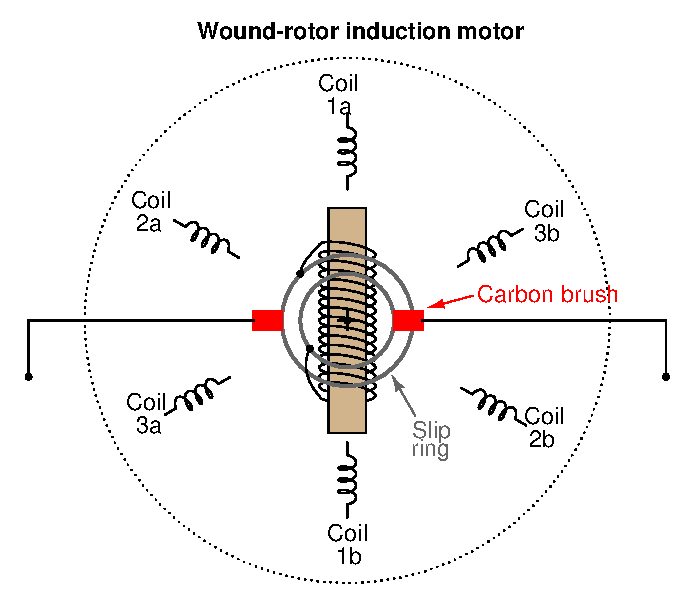
\includegraphics[width=15.5cm]{i01231x01.eps}$$

Når den eksterne kretsen er åpen, vil motoren ikke rotere. Når kretsen kortsluttes, oppfører motoren seg som en vanlig kortslutningsankermotor. Når kretsen eksiteres med likestrøm (DC), blir motoren en {\it synkronmotor}.

\vskip 10pt

Forklar hvordan denne motoren kan operere i disse ulike modusene, med utgangspunkt i generelle prinsipper for AC-motorer som Lenz' lov. Beskriv også hvordan motoren vil oppføre seg dersom en elektrisk motstand kobles mellom de to børsteterminalene, i stedet for åpen krets, kortslutning eller DC-eksitasjon.

\vskip 20pt \vbox{\hrule \hbox{\strut \vrule{} {\bf Forslag til sokratisk diskusjon} \vrule} \hrule}

\begin{itemize}
\item{} Identifiser et praktisk bruksområde for en viklet-rotor-motor.
\end{itemize}

\underbar{file i01231}
%(END_QUESTION)





%(BEGIN_ANSWER)

Hvis en motstand kobles inn i rotorkretsen, vil motoren oppføre seg som en ``svak'' induksjonsmotor: lavere hastighet og lavere moment enn med kortsluttet rotorvikling. Derfor ble viklet-rotor-induksjonsmotorer tidligere brukt mye i variable hastighetsapplikasjoner, siden hastighet og moment kunne justeres ved å endre motstandsverdien i rotorkretsen.
 
\vskip 10pt

Med åpen rotorvikling finnes ingen strømvei i rotoren. Lenz' lov får da ingen praktisk virkning fordi det ikke oppstår indusert {\it strøm} i rotorviklingen (selv om det fortsatt oppstår indusert {\it spenning}). Uten rotorstrøm oppstår heller ikke dreiemoment, og rotor vil derfor ikke rotere.

\vskip 10pt

Når rotorviklingen kortsluttes, blir den ekvivalent med permanent kortsluttet rotor i en ``squirrel-cage'' induksjonsmotor, og oppfører seg tilsvarende.

\vskip 10pt

Når rotorviklingen eksiteres med DC, får den en bestemt magnetisk polaritet og vil forsøke å følge statorens roterende magnetfelt i synkron hastighet.


%(END_ANSWER)





%(BEGIN_NOTES)


%INDEX% Elektronikkrepetisjon: drift av viklet-rotor-induksjonsmotor

%(END_NOTES)

